
%%%%%%%%%%%%%%%%%%%%%%%%%%%%%%%%%%%%%%%%%%%%%%%%%%%%%%%%%%%%%%%%%%%%%%%%%%%%%%%%%%%%%%%%%%
\begin{document}
\maketitle
%%%%%%%%%%%%%%%%%%%%%%%%%%%%%%%%%%%%%%%%%%%%%%%%%%%%%%%%%%%%%%%%%%%%%%%%%%%%%%%%%%%%%%%%%%

\begin{frame}
 \frametitle{Sumário}
  \vspace{-1cm}
  1. Introdução\\[0.1cm]
  2. Revisão Bibliográfica\\[0.1cm]
  3. Equações de Governo\\[0.1cm]
  4. Método dos Elementos Finitos\\[0.1cm]
  5. Validação do Código Numérico\\[0.1cm]
  6. Resultados\\[0.1cm]
  7. Conclusão
\end{frame}


%%%%%%%%%%%%%%%%%%%%%%%%%%%%%%%%%%%%%%%%%%%%%%%%%%%%%%%%%%%%%%%%%%%%%%%%%%%%%%%%%%%%%%%%%%

\begin{frame} 
\frametitle{Introdução - Motivação}
\begin{figure}
  \centering
  \vspace{-0.5cm}
  \includegraphics[scale=0.38]{images/corpo.jpg}
  \put(-240,210){Principais Causas de Morte no Mundo}
\end{figure}
\end{frame}

%%%%%%%%%%%%%%%%%%%%%%%%%%%%%%%%%%%%%%%%%%%%%%%%%%%%%%%%%%%%%%%%%%%%%%%%%%%%%%%%%%%%%%%%%%

\begin{frame} 
\frametitle{Introdução - Objetivos}
 \vspace{-1cm}
\begin{enumerate}
 \item Desenvolver um código em Elementos Finitos para a formulação 
    corrente-vorticidade com o transporte de espécie química \\

 \vspace{0.8cm}

 \item Conhecer a dinâmica do escoamento sanguíneo numa artéria coronária com aterosclerose
    e com stent farmacológico implantado
\end{enumerate}
\end{frame}

%%%%%%%%%%%%%%%%%%%%%%%%%%%%%%%%%%%%%%%%%%%%%%%%%%%%%%%%%%%%%%%%%%%%%%%%%%%%%%%%%%%%%%%%%%

\begin{frame}
  \vspace{-1cm}
  \textcolor{gray}{1. Introdução}\\[0.1cm]
  2. Revisão Bibliográfica\\[0.1cm]
  \textcolor{gray}{3. Equações de Governo}\\[0.1cm]
  \textcolor{gray}{4. Método dos Elementos Finitos}\\[0.1cm]
  \textcolor{gray}{5. Validação do Código Numérico}\\[0.1cm]
  \textcolor{gray}{6. Resultados}\\[0.1cm]
  \textcolor{gray}{7. Conclusão}
\end{frame}


%%%%%%%%%%%%%%%%%%%%%%%%%%%%%%%%%%%%%%%%%%%%%%%%%%%%%%%%%%%%%%%%%%%%%%%%%%%%%%%%%%%%%%%%%%

\begin{frame} 
\frametitle{Review - Stent Farmacológico}
\begin{figure}
  \vspace{-1.3cm}
  \includegraphics[scale=0.42]{images/stent_review.pdf}
\end{figure}
\end{frame}

%%%%%%%%%%%%%%%%%%%%%%%%%%%%%%%%%%%%%%%%%%%%%%%%%%%%%%%%%%%%%%%%%%%%%%%%%%%%%%%%%%%%%%%%%%

\begin{frame} 
\frametitle{Review - Stent Farmacológico}
  \vspace{-0.85cm}
\begin{figure}[H]
     \begin{minipage}{.50\linewidth}
      \centering
      \includegraphics[scale=0.3]{images/balloon.jpg}\\
      \scriptsize (a)
     \end{minipage}%
     \begin{minipage}{.50\linewidth}
      \centering
      \includegraphics[scale=0.3]{images/stent_bare.jpg}\\
      \scriptsize (b)
     \end{minipage}
\end{figure}
     \centering
     {\scriptsize Comparativo dos procedimentos PTCA:
              (a) balão inflável e
              (b) stent.}
\end{frame}


%%%%%%%%%%%%%%%%%%%%%%%%%%%%%%%%%%%%%%%%%%%%%%%%%%%%%%%%%%%%%%%%%%%%%%%%%%%%%%%%%%%%%%%%%%
\iffalse
\begin{frame} 
\frametitle{Review - Stent Farmacológico}
  \vspace{-0.85cm}
\begin{figure}[H]
     \begin{minipage}{.50\linewidth}
      \centering
      \includegraphics[scale=0.2]{images/stent_metal.jpg}\\
      \scriptsize (a)
     \end{minipage}%
     \begin{minipage}{.50\linewidth}
      \centering
      \includegraphics[scale=0.2]{images/stent_farmacologico.jpg}\\
      \scriptsize (b)
     \end{minipage}
\end{figure}
     \vspace{0.4cm}
     \centering
     {\scriptsize Comparativo das seções transversais:
              (a) stent e
              (b) stent farmacológico.}
\end{frame}
\fi
%%%%%%%%%%%%%%%%%%%%%%%%%%%%%%%%%%%%%%%%%%%%%%%%%%%%%%%%%%%%%%%%%%%%%%%%%%%%%%%%%%%%%%%%%%

\begin{frame} 
\frametitle{\Large Review - Método dos Elementos Finitos}
\begin{figure}
  \vspace{-1cm}
  \includegraphics[scale=0.4]{images/mef_review.pdf}
\end{figure}
\end{frame}

%%%%%%%%%%%%%%%%%%%%%%%%%%%%%%%%%%%%%%%%%%%%%%%%%%%%%%%%%%%%%%%%%%%%%%%%%%%%%%%%%%%%%%%%%%

\begin{frame} 
 \frametitle{\Large Review - Método dos Elementos Finitos}
\vspace{-1cm}
\begin{center}
\begin{columns}[c]
\begin{column}{0.8\textwidth} 
\hspace{1cm} \textbf{Hipóteses:}\\[0.1cm] 
\hspace{1cm}  1. Fluido como um Meio Contínuo\\[0.1cm]
\hspace{1cm}  2. Fluido incompressível\\[0.1cm]
\hspace{1cm}  3. Fluido newtoniano\\[0.1cm]
\hspace{1cm}  4. Escoamento monofásico\\[0.1cm]
\hspace{1cm}  5. Escoamento bidimensional\\[0.1cm]
\hspace{1cm}  6. Elevado número de Reynolds ($Re = \infty$)
\end{column}
\begin{column}{0.5\textwidth}
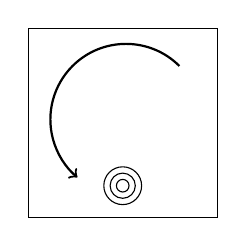
\begin{tikzpicture}[scale=0.8]
 \draw (0,0) -- (3,0) -- (3,3) -- (0,3) -- cycle;

 \draw [->,thick] (2.4,2.4) arc (45:230:1.2);

% \draw [->,thick] (-2,-0.1)--(-2,1.5) node[left] {$y$};
% \draw [->,thick] (-2.1,0)--(-0.5,0) node[below] {$x$};

 \draw (1.5,0.5) circle (0.3);
 \draw (1.5,0.5) circle (0.2);
 \draw (1.5,0.5) circle (0.1);
\end{tikzpicture}
\end{column}
\end{columns}
\end{center}
\vspace{0.5cm}
\begin{equation*}
 \frac{\partial c}{\partial t} 
 + 
 \textbf{v} \cdot \nabla c
 = 0
\end{equation*}
\end{frame}


%%%%%%%%%%%%%%%%%%%%%%%%%%%%%%%%%%%%%%%%%%%%%%%%%%%%%%%%%%%%%%%%%%%%%%%%%%%%%%%%%%%%%%%%%%

\begin{frame}
 \centering
 \vspace{-1cm}
 \Huge Video
\end{frame}

%%%%%%%%%%%%%%%%%%%%%%%%%%%%%%%%%%%%%%%%%%%%%%%%%%%%%%%%%%%%%%%%%%%%%%%%%%%%%%%%%%%%%%%%%%

\begin{frame}
  \vspace{-1cm}
  \textcolor{gray}{1. Introdução}\\[0.1cm]
  \textcolor{gray}{2. Revisão Bibliográfica}\\[0.1cm]
  3. Equações de Governo\\[0.1cm]
  \textcolor{gray}{4. Método dos Elementos Finitos}\\[0.1cm]
  \textcolor{gray}{5. Validação do Código Numérico}\\[0.1cm]
  \textcolor{gray}{6. Resultados}\\[0.1cm]
  \textcolor{gray}{7. Conclusão}
\end{frame}


%%%%%%%%%%%%%%%%%%%%%%%%%%%%%%%%%%%%%%%%%%%%%%%%%%%%%%%%%%%%%%%%%%%%%%%%%%%%%%%%%%%%%%%%%%

\begin{frame} 
 \frametitle{\Large Equações de Governo}
\vspace{-1cm}
\begin{center}
\begin{columns}[c]
\begin{column}{0.8\textwidth} 
\hspace{1cm} \textbf{Hipóteses:}\\[0.2cm] 
\hspace{1cm}  1. Fluido como um Meio Contínuo\\[0.1cm]
\hspace{1cm}  2. Fluido incompressível\\[0.1cm]
\hspace{1cm}  3. Fluido homogêneo e isotrópico\\[0.1cm]
\hspace{1cm}  4. Fluido newtoniano\\[0.1cm]
\hspace{1cm}  5. Fluido com difusividade de massa constante\\[0.1cm]
\hspace{1cm}  6. Escoamento monofásico\\[0.1cm]
\hspace{1cm}  7. Escoamento sem geração de espécie química
\end{column}
\begin{column}{0.5\textwidth}
\end{column}
\end{columns}
\end{center}
\small
\vspace{0cm}
\begin{equation*}
 \nabla \cdot \textbf{v}
 = 0 
\end{equation*}
\vspace{-0.3cm}
\begin{equation*}
 \frac{\partial \textbf{v}}{\partial t} + \textbf{v} \cdot \nabla \textbf{v}
 =
 -
 \frac{1}{\rho} \nabla p
 +
 \nu \nabla^{2} \textbf{v}
 +
 \textbf{g}
\end{equation*}
\vspace{-0.3cm}
\begin{equation*}
 \frac{\partial c}{\partial t}
 +
 \textbf{v} \cdot \nabla c
 =
 D \nabla^{2} c
\end{equation*}
\end{frame}

%%%%%%%%%%%%%%%%%%%%%%%%%%%%%%%%%%%%%%%%%%%%%%%%%%%%%%%%%%%%%%%%%%%%%%%%%%%%%%%%%%%%%%%%%%

\iffalse
\begin{frame} 
 \frametitle{\Large Equações de Governo}
\vspace{-1cm}
\begin{equation*}
 \nabla \cdot \textbf{v}
 = 0 
\end{equation*}
\vspace{0.3cm}
\begin{equation*}
 \frac{\partial \textbf{v}}{\partial t} + \textbf{v} \cdot \nabla \textbf{v}
 =
 -
 \frac{1}{\rho} \nabla p
 +
 \nu \nabla^{2} \textbf{v}
 +
 \textbf{g}
\end{equation*}
\vspace{0.3cm}
\begin{equation*}
 \frac{\partial c}{\partial t}
 +
 \textbf{v} \cdot \nabla c
 =
 D \nabla^{2} c
\end{equation*}
\end{frame}
\fi

%%%%%%%%%%%%%%%%%%%%%%%%%%%%%%%%%%%%%%%%%%%%%%%%%%%%%%%%%%%%%%%%%%%%%%%%%%%%%%%%%%%%%%%%%%

\begin{frame} 
 \frametitle{\Large Equações de Governo - Adimensionalização}
\vspace{-1cm}
\scriptsize
\begin{equation*}
 \begin{aligned}
  p & = \rho_{0} U^{2} p^{*} \\[10pt]
 \textbf{v} & = U \textbf{v}^{*} \\
 \end{aligned}
 \qquad
 \begin{aligned}
 c & = ( c_{s} - c_{0} ) c^{*} + c_{0}\\[10pt]
 \textbf{g} & = g_{0} \textbf{g}^{*} \\
 \end{aligned}
 \qquad
 \begin{aligned}
 \nu & = \nu_{0} \nu^{*} \\[10pt]
 \rho & = \rho_{0} \rho^{*} \\
 \end{aligned}
 \qquad
 \begin{aligned}
 D & = D_{0} D^{*} \\[5pt]
 \nabla & = \frac{1}{L} \nabla^{*} \\
 \end{aligned}
 \qquad
 \begin{aligned}
 x & = L x^{*} \\[5pt]
 t & = \frac{L}{U} t^{*} \\
 \end{aligned}
 \nonumber
\end{equation*}

\small
\vspace{1cm}
\begin{equation*}
 \nabla \cdot \textbf{v} = 0
\end{equation*}
\vspace{0.3cm}
\begin{equation*}
 \frac{\partial \textbf{v}}{\partial t} 
 + 
 \textbf{v} \cdot \nabla \textbf{v}
 =
 -
 \nabla p
 +
 \frac{1}{Re} \nabla^{2} \textbf{v}
 +
 \frac{1}{Fr^{2}} \textbf{g}
\end{equation*}
\vspace{0.3cm}
\begin{equation*}
 \frac{\partial c}{\partial t}
 +
 \textbf{v} \cdot \nabla c
 =
 \frac{1}{ReSc} \nabla^{2} c
\end{equation*}
\end{frame}

%%%%%%%%%%%%%%%%%%%%%%%%%%%%%%%%%%%%%%%%%%%%%%%%%%%%%%%%%%%%%%%%%%%%%%%%%%%%%%%%%%%%%%%%%%

\begin{frame} 
 \frametitle{\normalsize Equações de Governo - Formulação Corrente-Vorticidade}
\vspace{-1cm}
\scriptsize
\begin{equation*}
 \textbf{v} \cdot \nabla \textbf{v}
 = 
 \nabla \frac{v^{2}}{2}
 - 
 \textbf{v} \times \nabla \times \textbf{v}
 \hspace{1.2cm}
 \nabla \times \big[ \textbf{v} \times \omega \big]
 =
 -
 \textbf{v} \cdot \nabla \omega
 +
 \omega \cdot \nabla v
\end{equation*}

\small
\vspace{0.5cm}
\begin{equation*}
 \frac{\partial \omega}{\partial t} + \textbf{v} \cdot \nabla \omega = \frac{1}{Re} \nabla^{2} \omega
\end{equation*}
\vspace{0.2cm}
\begin{equation*}
\nabla^{2} \psi = - \omega
\end{equation*}
\vspace{0.2cm}
\begin{equation*}
\textbf{v} = \textbf{D} \psi
\end{equation*}
\vspace{0.2cm}
\begin{equation*}
\frac{\partial c}{\partial t} + \textbf{v} \cdot \nabla c = \frac{1}{ReSc} \nabla^{2} c
\end{equation*}\\[0.5cm]
Onde \textbf{D} é um operador diferencial
cujas componentes são $\big[\partial / \partial y,- \partial / \partial x \big]$
\end{frame}

%%%%%%%%%%%%%%%%%%%%%%%%%%%%%%%%%%%%%%%%%%%%%%%%%%%%%%%%%%%%%%%%%%%%%%%%%%%%%%%%%%%%%%%%%%

\begin{frame}
  \vspace{-1cm}
  \textcolor{gray}{1. Introdução}\\[0.1cm]
  \textcolor{gray}{2. Revisão Bibliográfica}\\[0.1cm]
  \textcolor{gray}{3. Equações de Governo}\\[0.1cm]
  4. Método dos Elementos Finitos\\[0.1cm]
  \textcolor{gray}{5. Validação do Código Numérico}\\[0.1cm]
  \textcolor{gray}{6. Resultados}\\[0.1cm]
  \textcolor{gray}{7. Conclusão}
\end{frame}


%%%%%%%%%%%%%%%%%%%%%%%%%%%%%%%%%%%%%%%%%%%%%%%%%%%%%%%%%%%%%%%%%%%%%%%%%%%%%%%%%%%%%%%%%%

\begin{frame} 
 \frametitle{\Large MEF - Discretização no tempo}
\vspace{-1cm}
\small
\begin{equation*}
\overset{.}{\omega} + \textbf{v}.\nabla \omega^n = \frac{1}{Re} \nabla^2 \omega^n 
 + \frac{\Delta t}{2} \textbf{v} \cdot \nabla \big[ \textbf{v} \cdot \nabla \omega^n \big]
\end{equation*}

\vspace{0.3cm}
\begin{equation*}
\nabla^2 \psi = - \omega
\end{equation*}

\vspace{0.3cm}
\begin{equation*}
\textbf{v} = \textbf{D}\psi
\end{equation*}

\vspace{0.3cm}
\begin{equation*}
\overset{.}{c} + \textbf{v}.\nabla c^n = \frac{1}{ReSc} \nabla^2 c^n
 + \frac{\Delta t}{2} \textbf{v} \cdot \nabla \big[ \textbf{v} \cdot \nabla c^n \big]
\end{equation*}

\scriptsize
\vspace{1cm}
Onde $\overset{.}{\omega}$ e
$\overset{.}{c}$ são
$\big[ \omega^{n+1}-\omega^{n} \big] /\Delta t$ e
$\big[ c^{n+1}-c^{n} \big] /\Delta t$ respectivamente,
\textbf{v} é o vetor velocidade cujas componentes são
$ \textbf{v} = [u,v]$
e \textbf{D} é um operador matemático com componentes
$ \textbf{D} = [\partial/\partial y, -\partial/\partial x]$

\end{frame}

%%%%%%%%%%%%%%%%%%%%%%%%%%%%%%%%%%%%%%%%%%%%%%%%%%%%%%%%%%%%%%%%%%%%%%%%%%%%%%%%%%%%%%%%%%

\begin{frame} 
 \frametitle{\Large MEF - Forma Matricial}
\vspace{-1cm}
\small
\begin{equation*}
\begin{aligned}
 \frac{M}{\Delta t} \omega^{n+1} = \frac{M}{\Delta t} \omega^{n} - u \cdot G_x & \omega^{n} - v \cdot G_y \omega^{n} 
 - \frac{1}{\textit{Re}} \Big[ K_{xx} + K_{yy} \Big] \omega^{n}  
 \\[5pt]
 & - \frac{\Delta t}{2} u \Big[ u K_{xx} + v K_{yx} \Big] \omega^{n} 
 - \frac{\Delta t}{2} v \Big[ u K_{xy} + v K_{yy} \Big] \omega^{n} 
\end{aligned}
\end{equation*}

\vspace{0.2cm}
\begin{equation*}
 \Big[ K_{xx} + K_{yy} \Big] \psi = M \omega
\end{equation*}

\begin{equation*}
 Mu = G_y \psi
\end{equation*}

\begin{equation*}
 Mv = - G_x \psi
\end{equation*}

\vspace{-0.3cm}
\begin{equation*}
\begin{aligned}
 \frac{M}{\Delta t} c^{n+1} = \frac{M}{\Delta t} c^{n}  - u \cdot G_x & c^{n} - v \cdot G_y c^{n} 
 - \frac{1}{\textit{ReSc}} \Big[ K_{xx} + K_{yy} \Big] c^{n}  
 \\[5pt]
 & - \frac{\Delta t}{2} u \Big[ u K_{xx} + v K_{yx} \Big] c^{n} 
 - \frac{\Delta t}{2} v \Big[ u K_{xy} + v K_{yy} \Big] c^{n} 
\end{aligned}
\end{equation*}
\end{frame}

%%%%%%%%%%%%%%%%%%%%%%%%%%%%%%%%%%%%%%%%%%%%%%%%%%%%%%%%%%%%%%%%%%%%%%%%%%%%%%%%%%%%%%%%%%
\iffalse
\begin{frame}
  \vspace{-1cm}
  \textcolor{gray}{1. Introdução}\\[0.1cm]
  \textcolor{gray}{2. Revisão Bibliográfica}\\[0.1cm]
  \textcolor{gray}{3. Equações de Governo}\\[0.1cm]
  \textcolor{gray}{4. Método dos Elementos Finitos}\\[0.1cm]
  5. Código Numérico e Algoritmo de Solução\\[0.1cm]
  \textcolor{gray}{6. Validação do Código Numérico}\\[0.1cm]
  \textcolor{gray}{7. Resultados}\\[0.1cm]
  \textcolor{gray}{8. Conclusão}
\end{frame}
\fi

%%%%%%%%%%%%%%%%%%%%%%%%%%%%%%%%%%%%%%%%%%%%%%%%%%%%%%%%%%%%%%%%%%%%%%%%%%%%%%%%%%%%%%%%%%

\iffalse
\begin{frame} 
 \frametitle{\Large Código Numérico - UML}
\vspace{-0.8cm}
\scriptsize
\begin{center}
\begin{tikzpicture}[scale=0.5]
 \draw [rounded corners=10,line width=2pt] (0,0) rectangle ++(3,3);
 \draw [line width=2pt] (0,2.4) -- (3,2.4);
 \draw [line width=2pt] (0,1.6) -- (3,1.6);
 \node (TriSim) at (1.5,2.7) {TriSim};

 \draw [rounded corners=10,line width=2pt] (0,6) rectangle ++(3,3);
 \draw [line width=2pt] (0,8.4) -- (3,8.4);
 \draw [line width=2pt] (0,7.6) -- (3,7.6);
 \node (TriMesh) at (1.5,8.7) {TriMesh};

 \draw [rounded corners=10,line width=2pt] (6,0) rectangle ++(3,3);
 \draw [line width=2pt] (6,2.4) -- (9,2.4);
 \draw [line width=2pt] (6,1.6) -- (9,1.6);
 \node (InOut) at (7.5,2.7) {InOut};
 
 \draw [rounded corners=10,line width=2pt] (-6,0) rectangle ++(3,3);
 \draw [line width=2pt] (-6,2.4) -- (-3,2.4);
 \draw [line width=2pt] (-6,1.6) -- (-3,1.6);
 \node (triBC) at (-4.5,2.7) {TriBC};

 \draw [rounded corners=10,line width=2pt] (0,-6) rectangle ++(3,3);
 \draw [line width=2pt] (0,-3.6) -- (3,-3.6);
 \draw [line width=2pt] (0,-4.4) -- (3,-4.4);
 \node (TElement) at (1.5,-3.3) {TElement};

 \draw [rounded corners=10,line width=2pt] (6,-6) rectangle ++(3.5,3);
 \draw [line width=2pt] (6,-3.6) -- (9.5,-3.6);
 \draw [line width=2pt] (6,-4.4) -- (9.5,-4.4);
 \node (FEMLinElement) at (7.8,-3.3) {FEMLinElem};

 \draw [{Diamond}-,line width=2pt] (TriSim) -- (1.5,6);
 \draw [{Diamond}-,line width=2pt] (0,1.5) -- (-3,1.5);
 \draw [{Diamond}-,line width=2pt] (1.5,0) -- (1.5,-3);
 \draw [{Diamond}-,line width=2pt] (3,1.5) -- (6,1.5);
 \draw [<-,line width=2pt] (3,-4.5) -- (6,-4.5);
\end{tikzpicture}
\end{center}

\centering Diagrama de Classes Simplificado
\end{frame}

\fi
%%%%%%%%%%%%%%%%%%%%%%%%%%%%%%%%%%%%%%%%%%%%%%%%%%%%%%%%%%%%%%%%%%%%%%%%%%%%%%%%%%%%%%%%%%
\iffalse
\begin{frame} 
 \frametitle{\Large Código Numérico}
\vspace{-1.5cm}
\scriptsize
\begin{figure}
  \centering
  \vspace{-0.3cm}
  \includegraphics[scale=0.2]{images/tempo_processamento.jpg}
\end{figure}
\centering Tempo de processamento em relação a simulação numérica para malhas triangulares lineares não estruturadas
\end{frame}
\fi

%%%%%%%%%%%%%%%%%%%%%%%%%%%%%%%%%%%%%%%%%%%%%%%%%%%%%%%%%%%%%%%%%%%%%%%%%%%%%%%%%%%%%%%%%%

\begin{frame} 
 \frametitle{\Large MEF - Algoritmo de Solução}
\vspace{-1cm}
% Define block styles
\tikzstyle{block} = [rectangle, draw,
    text width=27em, text centered, rounded corners, fill=gray!45!,scale=0.75,text=black!90!]
\tikzstyle{line} = [draw, -latex',scale=0.75]

\begin{center}
\begin{tikzpicture}[node distance = 1cm, auto]
    % Place nodes
    \node [block] (step1) {inicializar a vorticidade};
    \node [block, below of=step1] (step2) {inicializar a função de corrente};
    \node [block, below of=step2] (step3) {Calcular as condições de contorno da vorticidade};
    \node [block, below of=step3] (step4) {Calcular a vorticidade};
    \node [block, below of=step4] (step5) {Calcular a função de corrente};
    \node [block, below of=step5] (step6) {Calcular a velocidade};
    \node [block, below of=step6] (step7) {Calcular a concentração};
    \node [draw=none, align=center,scale=0.7,text=black!80!] at (6,-3) {Repetir o procedimento \\ para o próximo passo \\ de tempo};
    % Draw edges
    \path [line] (step1) -- (step2);
    \path [line] (step2) -- (step3);
    \path [line] (step3) -- (step4);
    \path [line] (step4) -- (step5);
    \path [line] (step5) -- (step6);
    \path [line] (step6) -- (step7);
    \path [line,dashed] (step7) -- (6,-6) |- (step3);
\end{tikzpicture}
\end{center}
\vspace{0.5cm}
\centering \scriptsize Algoritmo de solução da formulação corrente-vorticidade com transporte de espécie química
\end{frame}

%%%%%%%%%%%%%%%%%%%%%%%%%%%%%%%%%%%%%%%%%%%%%%%%%%%%%%%%%%%%%%%%%%%%%%%%%%%%%%%%%%%%%%%%%%

\begin{frame}
  \vspace{-1cm}
  \textcolor{gray}{1. Introdução}\\[0.1cm]
  \textcolor{gray}{2. Revisão Bibliográfica}\\[0.1cm]
  \textcolor{gray}{3. Equações de Governo}\\[0.1cm]
  \textcolor{gray}{4. Método dos Elementos Finitos}\\[0.1cm]
  5. Validação do Código Numérico\\[0.1cm]
  \textcolor{gray}{6. Resultados}\\[0.1cm]
  \textcolor{gray}{7. Conclusão}
\end{frame}


%%%%%%%%%%%%%%%%%%%%%%%%%%%%%%%%%%%%%%%%%%%%%%%%%%%%%%%%%%%%%%%%%%%%%%%%%%%%%%%%%%%%%%%%%%

\begin{frame}
 \frametitle{\small Validação do Código Numérico - Escoamento de Couette}
\vspace{-1cm}
\begin{center}
\begin{tikzpicture}[scale=1]
 \draw [pattern=north east lines] (0,0) -- (0,-0.1) -- (5,-0.1) -- (5,0) -- cycle;
 \draw [pattern=north east lines] (0,1) -- (0,1.1) -- (5,1.1) -- (5,1) -- cycle;

 \draw [->,thick] (5.1,1)--(6,1) node[above] {$U_{top}$};
 \draw [->,thick] (-0.1,0)--(-1,0) node[below] {$U_{bottom}$};

% \draw [->,thick] (-4,-0.1)--(-4,1.5) node[left] {$y$};
% \draw [->,thick] (-4.1,0)--(-2.5,0) node[below] {$x$};

 \draw [dotted] (2.5,0.0) to (2.5,1.0);
 \draw  (1.5,0.0) to (3.5,1.0);

 \draw [->,thick] (2.5,0.0) to (1.5,0.0);
 \draw [->,thick] (2.5,0.15) to (1.8,0.15);
 \draw [->,thick] (2.5,0.35) to (2.2,0.35);

 \draw [->,thick] (2.5,1) to (3.5,1);
 \draw [->,thick] (2.5,0.85) to (3.2,0.85);
 \draw [->,thick] (2.5,0.65) to (2.8,0.65);
\end{tikzpicture}
\end{center}
\vspace{0.5cm}
\small
As condições de contorno são:\\[0.2cm]
Placa Superior: $u=U_{top}$ onde $U_{top} = 1$, $v=0$ e $\psi=0$;\\[0.1cm]
Placa Inferior: $u=U_{bottom}$ onde $U_{bottom} = -1$, $v=0$ e $\psi=0$
\vspace{0.5cm}
\begin{equation*}
 u = \big[ U_{top} - U_{bottom} \big] \frac{y}{L} + U_{bottom}
\end{equation*}
\end{frame}

%%%%%%%%%%%%%%%%%%%%%%%%%%%%%%%%%%%%%%%%%%%%%%%%%%%%%%%%%%%%%%%%%%%%%%%%%%%%%%%%%%%%%%%%%%

\begin{frame} 
 \frametitle{\small Validação do Código Numérico - Escoamento de Couette}
\begin{figure}
  \centering
  \vspace{-1.5cm}
  \includegraphics[scale=0.6]{images/couette_velocity.pdf}
\end{figure}
\vspace{-0.2cm}
\centering \scriptsize Evolução do perfil de velocidade no tempo para Re = 100 e a comparação da
solução numérica com a solução analítica.
\end{frame}

%%%%%%%%%%%%%%%%%%%%%%%%%%%%%%%%%%%%%%%%%%%%%%%%%%%%%%%%%%%%%%%%%%%%%%%%%%%%%%%%%%%%%%%%%%

\begin{frame}
 \frametitle{\small Validação do Código Numérico - Escoamento de Poiseuille}
\vspace{-1cm}
\begin{center}
\begin{tikzpicture}[scale=1]
 \draw [pattern=north east lines] (0,0) -- (0,-0.1) -- (5,-0.1) -- (5,0) -- cycle;
 \draw [pattern=north east lines] (0,1) -- (0,1.1) -- (5,1.1) -- (5,1) -- cycle;

% \draw [->,thick] (-2,-0.1)--(-2,1.5) node[left] {$y$};
% \draw [->,thick] (-2.1,0)--(-0.5,0) node[below] {$x$};

 \draw [dotted] (2.5,0.0) to (2.5,1.0);
 \draw  (2.5,0.0) to [bend right=100] (2.5,1.0);

 \draw [->,thick] (2.5,0.9) to (2.7,0.9);
 \draw [->,thick] (2.5,0.7) to (2.78,0.7);
 \draw [->,thick] (2.5,0.5) to (2.8,0.5);
 \draw [->,thick] (2.5,0.3) to (2.78,0.3);
 \draw [->,thick] (2.5,0.1) to (2.7,0.1);
\end{tikzpicture}
\end{center}
\vspace{0.5cm}
\small
As condições de contorno são:\\[0.2cm]
Condição de Entrada: $u=1$, $v=0$ e $\psi=y$;\\[0.1cm]
Condição de Saida: $\psi=y$;\\[0.1cm]
Parede superior: $u=0$, $v=0$, $\psi=1$;\\[0.1cm]
Parede inferior: $u=0$, $v=0$, $\psi=0$
\vspace{0.5cm}
\begin{equation*}
u = \frac{4 u_{max}}{L^2} y \big[ L - y \big]
\end{equation*}
\end{frame}

%%%%%%%%%%%%%%%%%%%%%%%%%%%%%%%%%%%%%%%%%%%%%%%%%%%%%%%%%%%%%%%%%%%%%%%%%%%%%%%%%%%%%%%%%%

\begin{frame}
 \frametitle{\small Validação do Código Numérico - Escoamento de Poiseuille}
\begin{figure}
  \centering
  \vspace{-1.5cm}
  \includegraphics[scale=0.6]{images/poiseuille_velocity.pdf}
\end{figure}
\vspace{-0.2cm}
\centering \scriptsize Evolução do perfil de velocidade no tempo para Re = 100 e a comparação da
solução numérica com a solução analítica.
\end{frame}

%%%%%%%%%%%%%%%%%%%%%%%%%%%%%%%%%%%%%%%%%%%%%%%%%%%%%%%%%%%%%%%%%%%%%%%%%%%%%%%%%%%%%%%%%%

\iffalse
\begin{frame}
 \frametitle{\small Validação do Código Numérico - Escoamento em Meio Domínio}
\vspace{-1cm}
\begin{center}
\begin{tikzpicture}[scale=1]
 \draw [pattern=north east lines] (0,1) -- (0,1.1) -- (5,1.1) -- (5,1) -- cycle;
 \draw [dashed] (-0.3,0.0) to (5.3,0.0);

% \draw [->,thick] (-2,-0.1)--(-2,1.5) node[left] {$y$};
% \draw [->,thick] (-2.1,0)--(-0.5,0) node[below] {$x$};

 \draw [->,thick] (5.4,0.0)--(6.1,0.0);
 \node [draw=none] at (7.1,0.0) {$simetria$};

 \draw [dotted] (2.5,0.0) to (2.5,1.0);
 \draw  (2.8,0.0) to [bend right=20] (2.5,1.0);

 \draw [->,thick] (2.5,0.0) to (2.8,0.0);
 \draw [->,thick] (2.5,0.3) to (2.78,0.3);
 \draw [->,thick] (2.5,0.6) to (2.71,0.6);
 \draw [->,thick] (2.5,0.85) to (2.6,0.85);
\end{tikzpicture}
\end{center}
\vspace{0.5cm}
\small
As condições de contorno são:\\[0.2cm]
Condição de Entrada: $u=1$, $v=0$ e $\psi=y$;\\[0.1cm]
Condição de Saida: $\psi=y$;\\[0.1cm]
Parede superior: $u=0$, $v=0$, $\psi=1$;\\[0.1cm]
Eixo de simetria: $v=0$, $\psi=0$
\vspace{0.5cm}
\begin{equation*}
u = u_{max} \big[ 1 - \frac{y^{2}}{L^{2}} \big]
\end{equation*}
\end{frame}
\fi

%%%%%%%%%%%%%%%%%%%%%%%%%%%%%%%%%%%%%%%%%%%%%%%%%%%%%%%%%%%%%%%%%%%%%%%%%%%%%%%%%%%%%%%%%%

\iffalse
\begin{frame}
 \frametitle{\small Validação do Código Numérico - Escoamento em Meio Domínio}
\begin{figure}
  \centering
  \vspace{-1.5cm}
  \includegraphics[scale=0.6]{images/half_poiseuille_velocity.pdf}
\end{figure}
\vspace{-0.2cm}
\centering \scriptsize Evolução do perfil de velocidade no tempo para Re = 100 e a comparação da
solução numérica com a solução analítica.
\end{frame}
\fi

%%%%%%%%%%%%%%%%%%%%%%%%%%%%%%%%%%%%%%%%%%%%%%%%%%%%%%%%%%%%%%%%%%%%%%%%%%%%%%%%%%%%%%%%%%

\begin{frame}
 \frametitle{\small Validação do Código Numérico - Escoamento em Cavidade}
\vspace{-1cm}
\begin{center}
\begin{tikzpicture}[scale=0.8]
\draw [pattern=north east lines] (0,-0.1) -- (3,-0.1) -- (3,3) -- (2.9,3) -- (2.9,0) -- (0.1,0) -- (0.1,3) -- (0,3) -- cycle;
 \draw [pattern=north east lines] (-0.1,3) -- (-0.1,3.1) -- (3.1,3.1) -- (3.1,3) -- cycle;

 \draw [->,thick] (3.2,3.05)--(4.2,3.05) node[above] {$U_{top}$};

 \draw [->,thick] (2.4,2.4) arc (45:-180:1.2);

% \draw [->,thick] (-2,-0.1)--(-2,1.5) node[left] {$y$};
% \draw [->,thick] (-2.1,0)--(-0.5,0) node[below] {$x$};
\end{tikzpicture}
\end{center}
\vspace{0.5cm}
\small
As condições de contorno são:\\[0.2cm]
Paredes laterais e inferior: $u=0$, $v=0$ e $\psi=0$;\\[0.1cm]
Parede superior: $u=1$, $v=0$ e $\psi=0$
\end{frame}

%%%%%%%%%%%%%%%%%%%%%%%%%%%%%%%%%%%%%%%%%%%%%%%%%%%%%%%%%%%%%%%%%%%%%%%%%%%%%%%%%%%%%%%%%%

\begin{frame}
 \frametitle{\small Validação do Código Numérico - Escoamento em Cavidade}
\begin{figure}
  \centering
  \vspace{-1.5cm}
  \includegraphics[scale=0.6]{images/Re_100_u_profile.pdf}
\end{figure}
\vspace{-0.2cm}
\centering \scriptsize Perfil de $u$ na linha central da cavidade ($x=0.5$) para Reynolds $Re=100$.
\end{frame}

%%%%%%%%%%%%%%%%%%%%%%%%%%%%%%%%%%%%%%%%%%%%%%%%%%%%%%%%%%%%%%%%%%%%%%%%%%%%%%%%%%%%%%%%%%

\begin{frame}
 \frametitle{\small Validação do Código Numérico - Escoamento em Cavidade}
\begin{figure}
  \centering
  \vspace{-1.5cm}
  \includegraphics[scale=0.6]{images/Re_100_v_profile.pdf}
\end{figure}
\vspace{-0.2cm}
\centering \scriptsize Perfil de $v$ na linha central da cavidade ($y=0.5$) para Reynolds $Re=100$.
\end{frame}

%%%%%%%%%%%%%%%%%%%%%%%%%%%%%%%%%%%%%%%%%%%%%%%%%%%%%%%%%%%%%%%%%%%%%%%%%%%%%%%%%%%%%%%%%%

\begin{frame}
  \vspace{-1cm}
  \textcolor{gray}{1. Introdução}\\[0.1cm]
  \textcolor{gray}{2. Revisão Bibliográfica}\\[0.1cm]
  \textcolor{gray}{3. Equações de Governo}\\[0.1cm]
  \textcolor{gray}{4. Método dos Elementos Finitos}\\[0.1cm]
  \textcolor{gray}{5. Validação do Código Numérico}\\[0.1cm]
  6. Resultados\\[0.1cm]
  \textcolor{gray}{7. Conclusão}
\end{frame}


%%%%%%%%%%%%%%%%%%%%%%%%%%%%%%%%%%%%%%%%%%%%%%%%%%%%%%%%%%%%%%%%%%%%%%%%%%%%%%%%%%%%%%%%%%

\begin{frame}
 \frametitle{\Large Resultados}
\begin{figure}
  \vspace{-1cm}
     \centering
     \begin{minipage}{.45\linewidth}
      \centering
      \includegraphics[scale=0.15]{images/CurvedStrut.png}\\
      \scriptsize (a)
     \end{minipage}%
     \begin{minipage}{.45\linewidth}
      \centering
      \includegraphics[scale=0.15]{images/RealStrut.png}\\
      \scriptsize (b)
     \end{minipage}
\end{figure}
\vspace{-0.3cm}
\begin{center}
\scriptsize 
     Geometria não dimensional para escoamento sanguíneao em artéria coronária.
     (a) Canal Curvado com Stent
     (b) Canal Real com Stent.
\end{center}
\vspace{0.05cm}
\small
\begin{center}
\begin{columns}[c]
\begin{column}{0.8\textwidth} 
As condições de contorno são:\\[0.2cm]
Condição de Entrada: $u=1$, $v=0$ e $\psi=y$;\\[0.1cm]
Condição de Saida: $\psi=y$;\\[0.1cm]
Parede superior: $u=0$, $v=0$, $\psi=1$;\\[0.1cm]
Eixo de simetria: $v=0$, $\psi=0$; \\[0.1cm]
Stent Farmacológico: $u=0$, $v=0$, $\psi=1$ e $c=1$
\end{column}
\hspace{-1cm}
\begin{column}{0.3\textwidth}
$R=0.0015m$\\[0.1cm]
$\mu=0.0035Pa.s$\\[0.1cm]
$\rho=1060kg/m^3$\\[0.1cm]\\
$u=12cm/s$\\[0.1cm]
$Re=54.5$
\end{column}
\end{columns}
\end{center}
\end{frame}

%%%%%%%%%%%%%%%%%%%%%%%%%%%%%%%%%%%%%%%%%%%%%%%%%%%%%%%%%%%%%%%%%%%%%%%%%%%%%%%%%%%%%%%%%%

\begin{frame}
 \frametitle{\Large Resultados - Canal Curvado com Stent}
\begin{figure}
     \begin{minipage}{.50\linewidth}
      \centering
      \includegraphics[scale=0.08]{images/vel_CurvedStrut200.png}\\
      \scriptsize t = 0.1
     \end{minipage}%
     \begin{minipage}{.50\linewidth}
      \centering
      \includegraphics[scale=0.08]{images/vel_CurvedStrut1000.png}\\
      \scriptsize t = 0.5
     \end{minipage}
     \begin{minipage}{.50\linewidth}
     \medskip
      \centering
      \includegraphics[scale=0.08]{images/vel_CurvedStrut2000.png}\\
      \scriptsize t = 1.0
     \end{minipage}%
     \begin{minipage}{.50\linewidth}
     \medskip
      \centering
      \includegraphics[scale=0.08]{images/vel_CurvedStrut6000.png}\\
      \scriptsize t = 3.0
     \end{minipage}
     \begin{minipage}{.50\linewidth}
      \centering
      \includegraphics[scale=0.08]{images/vel_CurvedStrut8000.png}\\
      \scriptsize t = 4.0
     \end{minipage}%
     \begin{minipage}{.50\linewidth}
      \centering
      \includegraphics[scale=0.08]{images/vel_CurvedStrut10000.png}\\
      \scriptsize t = 5.0
 \end{minipage}
     \begin{minipage}{.50\linewidth}
     \medskip
      \centering
      \includegraphics[scale=0.08]{images/vel_CurvedStrut14000.png}\\
      \scriptsize t = 7.0
     \end{minipage}%
     \begin{minipage}{.50\linewidth}
     \medskip
      \centering
      \includegraphics[scale=0.08]{images/vel_CurvedStrut20000.png}\\
      \scriptsize t = 10.0
     \end{minipage}
\end{figure}
\vspace{0cm}
\centering \scriptsize Evolução no tempo e no espaço do campo de velocidade para o Canal Curvado com Stent Farmacológico
\end{frame}


%%%%%%%%%%%%%%%%%%%%%%%%%%%%%%%%%%%%%%%%%%%%%%%%%%%%%%%%%%%%%%%%%%%%%%%%%%%%%%%%%%%%%%%%%%

\begin{frame}
 \frametitle{\Large Resultados - Canal Curvado com Stent}
\begin{figure}
  \centering
  \vspace{-1.5cm}
  \includegraphics[scale=0.59]{images/vel_CurvedStrut_evol.pdf}\\
\end{figure}
\vspace{-0.2cm}
\centering \scriptsize Evolução no tempo do perfil da velocidade para o Canal Curvado com Stent Farmacológico
\end{frame}

%%%%%%%%%%%%%%%%%%%%%%%%%%%%%%%%%%%%%%%%%%%%%%%%%%%%%%%%%%%%%%%%%%%%%%%%%%%%%%%%%%%%%%%%%%

\begin{frame}
 \frametitle{\Large Resultados - Canal Curvado com Stent}
\begin{figure}
     \begin{minipage}{.50\linewidth}
      \centering
      \includegraphics[scale=0.08]{images/conc1_CurvedStrut1000.png}\\
      \scriptsize t = 0.5
     \end{minipage}%
     \begin{minipage}{.50\linewidth}
      \centering
      \includegraphics[scale=0.08]{images/conc1_CurvedStrut2000.png}\\
      \scriptsize t = 1.0
     \end{minipage}
     \begin{minipage}{.50\linewidth}
     \medskip
      \centering
      \includegraphics[scale=0.08]{images/conc1_CurvedStrut10000.png}\\
      \scriptsize t = 5.0
     \end{minipage}%
     \begin{minipage}{.50\linewidth}
     \medskip
      \centering
      \includegraphics[scale=0.08]{images/conc1_CurvedStrut20000.png}\\
      \scriptsize t = 10.0
     \end{minipage}
\end{figure}
\vspace{0cm}
\centering \scriptsize Canal Curvado com Stent Farmacológico cujo $Sc=1$.
\vspace{0.5cm}
\begin{figure}
     \begin{minipage}{.50\linewidth}
      \centering
      \includegraphics[scale=0.08]{images/conc10_CurvedStrut2500.png}\\
      \scriptsize t = 0.5
     \end{minipage}%
     \begin{minipage}{.50\linewidth}
      \centering
      \includegraphics[scale=0.08]{images/conc10_CurvedStrut5000.png}\\
      \scriptsize t = 1.0
     \end{minipage}
     \begin{minipage}{.50\linewidth}
     \medskip
      \centering
      \includegraphics[scale=0.08]{images/conc10_CurvedStrut25000.png}\\
      \scriptsize t = 5.0
     \end{minipage}%
     \begin{minipage}{.50\linewidth}
     \medskip
      \centering
      \includegraphics[scale=0.08]{images/conc10_CurvedStrut50000.png}\\
      \scriptsize t = 10.0
     \end{minipage}
\end{figure}
\vspace{0cm}
\centering \scriptsize Canal Curvado com Stent Farmacológico cujo $Sc=10$.
\end{frame}

%%%%%%%%%%%%%%%%%%%%%%%%%%%%%%%%%%%%%%%%%%%%%%%%%%%%%%%%%%%%%%%%%%%%%%%%%%%%%%%%%%%%%%%%%%

\begin{frame}
 \frametitle{\Large Resultados - Canal Real com Stent}
\begin{figure}
     \begin{minipage}{.50\linewidth}
      \centering
      \includegraphics[scale=0.08]{images/vel_RealStrut200.png}\\
      \scriptsize t = 0.1
     \end{minipage}%
     \begin{minipage}{.50\linewidth}
      \centering
      \includegraphics[scale=0.08]{images/vel_RealStrut1000.png}\\
      \scriptsize t = 0.5
     \end{minipage}
     \begin{minipage}{.50\linewidth}
     \medskip
      \centering
      \includegraphics[scale=0.08]{images/vel_RealStrut2000.png}\\
      \scriptsize t = 1.0
     \end{minipage}%
     \begin{minipage}{.50\linewidth}
     \medskip
      \centering
      \includegraphics[scale=0.08]{images/vel_RealStrut6000.png}\\
      \scriptsize t = 3.0
     \end{minipage}
     \begin{minipage}{.50\linewidth}
      \centering
      \includegraphics[scale=0.08]{images/vel_RealStrut8000.png}\\
      \scriptsize t = 4.0
     \end{minipage}%
     \begin{minipage}{.50\linewidth}
      \centering
      \includegraphics[scale=0.08]{images/vel_RealStrut10000.png}\\
      \scriptsize t = 5.0
 \end{minipage}
     \begin{minipage}{.50\linewidth}
     \medskip
      \centering
      \includegraphics[scale=0.08]{images/vel_RealStrut14000.png}\\
      \scriptsize t = 7.0
     \end{minipage}%
     \begin{minipage}{.50\linewidth}
     \medskip
      \centering
      \includegraphics[scale=0.08]{images/vel_RealStrut20000.png}\\
      \scriptsize t = 10.0
     \end{minipage}
\end{figure}
\vspace{0cm}
\centering \scriptsize Evolução no tempo e no espaço do campo de velocidade para o Canal Real com Stent Farmacológico
\end{frame}


%%%%%%%%%%%%%%%%%%%%%%%%%%%%%%%%%%%%%%%%%%%%%%%%%%%%%%%%%%%%%%%%%%%%%%%%%%%%%%%%%%%%%%%%%%

\begin{frame}
 \frametitle{\Large Resultados - Canal Real com Stent}
\begin{figure}
  \centering
  \vspace{-1.5cm}
  \includegraphics[scale=0.59]{images/vel_RealStrut_evol.pdf}\\
\end{figure}
\vspace{-0.2cm}
\centering \scriptsize Evolução no tempo do perfil da velocidade para o Canal Real com Stent Farmacológico
\end{frame}

%%%%%%%%%%%%%%%%%%%%%%%%%%%%%%%%%%%%%%%%%%%%%%%%%%%%%%%%%%%%%%%%%%%%%%%%%%%%%%%%%%%%%%%%%%

\begin{frame}
 \frametitle{\Large Resultados - Canal Real com Stent}
\begin{figure}
     \begin{minipage}{.50\linewidth}
      \centering
      \includegraphics[scale=0.08]{images/conc1_RealStrut1000.png}\\
      \scriptsize t = 0.5
     \end{minipage}%
     \begin{minipage}{.50\linewidth}
      \centering
      \includegraphics[scale=0.08]{images/conc1_RealStrut2000.png}\\
      \scriptsize t = 1.0
     \end{minipage}
     \begin{minipage}{.50\linewidth}
     \medskip
      \centering
      \includegraphics[scale=0.08]{images/conc1_RealStrut10000.png}\\
      \scriptsize t = 5.0
     \end{minipage}%
     \begin{minipage}{.50\linewidth}
     \medskip
      \centering
      \includegraphics[scale=0.08]{images/conc1_RealStrut20000.png}\\
      \scriptsize t = 10.0
     \end{minipage}
\end{figure}
\vspace{0cm}
\centering \scriptsize Canal Real com Stent Farmacológico cujo $Sc=1$.
\vspace{0.5cm}
\begin{figure}
     \begin{minipage}{.50\linewidth}
      \centering
      \includegraphics[scale=0.077]{images/conc10_RealStrut2500.png}\\
      \scriptsize t = 0.5
     \end{minipage}%
     \begin{minipage}{.50\linewidth}
      \centering
      \includegraphics[scale=0.077]{images/conc10_RealStrut5000.png}\\
      \scriptsize t = 1.0
     \end{minipage}
     \begin{minipage}{.50\linewidth}
     \medskip
      \centering
      \includegraphics[scale=0.077]{images/conc10_RealStrut25000.png}\\
      \scriptsize t = 5.0
     \end{minipage}%
     \begin{minipage}{.50\linewidth}
     \medskip
      \centering
      \includegraphics[scale=0.077]{images/conc10_RealStrut50000.png}\\
      \scriptsize t = 10.0
     \end{minipage}
\end{figure}
\vspace{0cm}
\centering \scriptsize Canal Real com Stent Farmacológico cujo $Sc=10$.
\end{frame}

%%%%%%%%%%%%%%%%%%%%%%%%%%%%%%%%%%%%%%%%%%%%%%%%%%%%%%%%%%%%%%%%%%%%%%%%%%%%%%%%%%%%%%%%%%

\begin{frame}
  \vspace{-1cm}
  \textcolor{gray}{1. Introdução}\\[0.1cm]
  \textcolor{gray}{2. Revisão Bibliográfica}\\[0.1cm]
  \textcolor{gray}{3. Equações de Governo}\\[0.1cm]
  \textcolor{gray}{4. Método dos Elementos Finitos}\\[0.1cm]
  \textcolor{gray}{5. Validação do Código Numérico}\\[0.1cm]
  \textcolor{gray}{6. Resultados}\\[0.1cm]
  7. Conclusão
\end{frame}


%%%%%%%%%%%%%%%%%%%%%%%%%%%%%%%%%%%%%%%%%%%%%%%%%%%%%%%%%%%%%%%%%%%%%%%%%%%%%%%%%%%%%%%%%%

\begin{frame}
 \frametitle{\Large Conclusão}
 \vspace{-1cm}
\begin{enumerate}
 \small
 \item Foi construído um código completo em linguagem de programação de alto nível (Python)
       usando o paradigma de orientação de objetos e partir do presente momento, possuímos
       uma plataforma de estudos de problemas de escoamento de fármacos em artérias\\

 \vspace{0.3cm}
 
 \item O simulador é capaz também de descrever em detalhes problemas envolvendo escoamento
       de fluidos newtonianos com transporte de natureza escalar (concentração ou temperatura)
       devido a construção generalizada do código\\

 \vspace{0.3cm}

 \item A formulação corrente-vorticidade se mostrou uma aproximação usual para
       calcular os campos de velocidade e concentração já que as variáveis são
       escalares permitindo uma implementação suave \\

 \vspace{0.3cm}
 
 \item Foi observado que o número de \textit{Schmidt} influencia diretamente no transporte do fármaco
       na corrente sanguínea. Para elevados valores de \textit{Schmidt}, o transporte de espécie química
       torna-se puramente convectivo e sua influência na parede da artéria deve ser verificada
\end{enumerate}
\end{frame}


%%%%%%%%%%%%%%%%%%%%%%%%%%%%%%%%%%%%%%%%%%%%%%%%%%%%%%%%%%%%%%%%%%%%%%%%%%%%%%%%%%%%%%%%%%

\begin{frame}
 \frametitle{\Large Conclusão - Trabalhos Futuros}
 \vspace{-1cm}
\begin{enumerate}
 \item Implementação do esquema Semi-Lagrangeano\\

 \vspace{0.8cm}
 
 \item Utilização das variáveis primitivas na equação Navier-Stokes numa abordagem 3D\\
 
 \vspace{0.8cm}

 \item Modelar o escoamento sanguíneo como um problema multifásico\\
 
 \vspace{0.8cm}

 \item Simular a transferência de espécie química na parede da artéria
\end{enumerate}
\end{frame}

%%%%%%%%%%%%%%%%%%%%%%%%%%%%%%%%%%%%%%%%%%%%%%%%%%%%%%%%%%%%%%%%%%%%%%%%%%%%%%%%%%%%%%%%%%

\begin{frame}
 \centering
 \vspace{-1cm}
 \Huge Obrigado!\\
 \vspace{0.5cm}
 \small marquesleandro67@gmail.com
\end{frame}




\end{document}
%%%%%%%%%%%%%%%%%%%%%%%%%%%%%%%%%%%%%%%%%%%%%%%%%%%%%%%%%%%%%%%%%%%%%%%%%%%%%%%%%%%%%%%%%%
